\documentclass{sem5}

\institutename{Indian Institute of Information Technology, Vadodara}
\author{Dilip Puri}
\idt{201351014}
%\team{teamname}
\collab{\textbf{Collaborator} - Hemant Kumar(201352026)}

\coursename{Parallel Programming}
\ccode{\begin{small}CS403\end{small}}
\profname{Prof. Reshmi Mitra}

\type{Lab}
\typeid{01}
\submissiondate{\today}%dd/mm/yyyy
\deadline{Due Aug 15, 4:00 PM}%dd/mm/yyyy @hh:mm pm/am
\problemset{Peak Performance, Basic Linux commands, Introduction to POSIX threads}

\begin{document}
\section*{Peak Performance}
\begin{enumerate}
\item[Problem 1] Consider a memory system with a level 1 cache of 32 KB and DRAM of 512 MB with the processor operating at 1 GHz. The latency to L1 cache is 1 cycle and the latency to DRAM is 100 cycles. In each memory cycle, the processor fetches four words (cache line size is 4 words). What is the peak achievable performance of a dot product of two vectors?
\lstset{language=C}
\begin{lstlisting}[frame=single]
/* dot product loop */
for (i = 0; i < dim; i++)
	dot_prod += a[i] * b[i];
\end{lstlisting}
\textbf{Answer}:
\lstset{language=C}
\begin{lstlisting}[frame=single]
/* dot product loop */
for (i = 0; i < dim; i++)
	dot_prod += a[i] * b[i];
\end{lstlisting}
\item[Problem 2] Now consider the problem of multiplying a dense matrix with a vector using a two-loop dot-product formulation. The matrix is of dimension 4K x 4K. (Each row of the matrix takes 16 KB of storage.) What is the peak achievable performance of this technique using a two-loop dot-product based matrix-vector product?
\lstset{language=C}
\begin{lstlisting}[frame=single]
/* matrix-vector product loop */
for (i = 0; i < dim; i++)
	for (j = 0; j < dim; j++)
		c[i] += a[i][j] * b[i];
\end{lstlisting}
\textbf{Answer}:
\lstset{language=C}
\begin{lstlisting}[frame=single]
/* dot product loop */

adf
adf
\end{lstlisting}
\end{enumerate}
\section*{Linux commands}
\lstset{language=C}
\begin{lstlisting}[frame=single]
$top
\end{lstlisting}
\begin{figure}[htp]
\centering
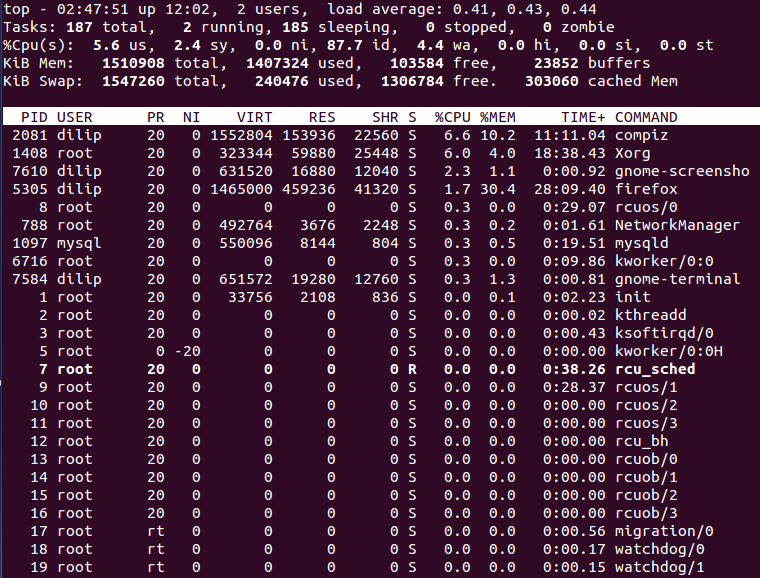
\includegraphics[scale=.4]{1.png}
\caption{top: provides dynamic real-time view of individual jobs running on the system}
\end{figure}
\begin{lstlisting}[frame=single]
$gnome-system-monitor
\end{lstlisting}
\begin{figure}[!htp]
\centering
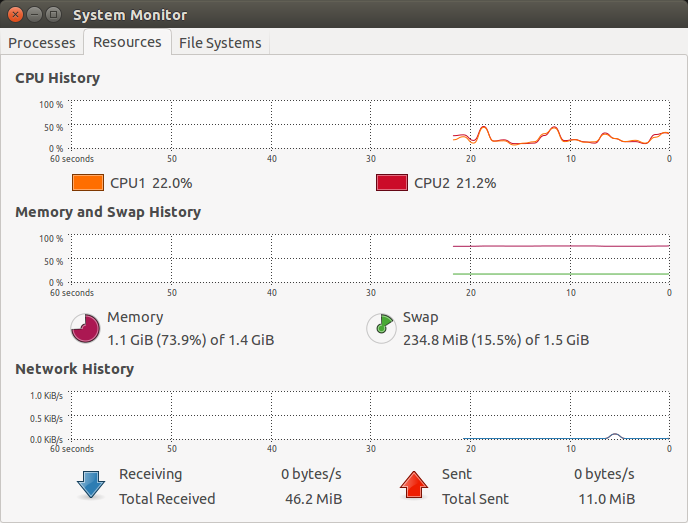
\includegraphics[scale=.5]{2.png}
\caption{gnome-system-monitor: shows which programs are running and how much processor time, memory, and disk space are being used. This gives an overall system view whereas the ``top" instruction represents a detailed perspective}
\end{figure}
\begin{lstlisting}[frame=single]
$lscpu
We can also get the same information from $cat /proc/cpuinfo 
==================================
Architecture:          x86_64
CPU op-mode(s):        32-bit, 64-bit
Byte Order:            Little Endian
CPU(s):                2
On-line CPU(s) list:   0,1
Thread(s) per core:    1
Core(s) per socket:    2
Socket(s):             1
NUMA node(s):          1
Vendor ID:             AuthenticAMD
CPU family:            18
Model:                 1
Stepping:              0
CPU MHz:               800.000
BogoMIPS:              4392.08
Virtualization:        AMD-V
L1d cache:             64K
L1i cache:             64K
L2 cache:              1024K
NUMA node0 CPU(s):     0,1
dilip@dilip-notebook-pc:~$ lscpu
Architecture:          x86_64
CPU op-mode(s):        32-bit, 64-bit
Byte Order:            Little Endian
CPU(s):                2
On-line CPU(s) list:   0,1
Thread(s) per core:    1
Core(s) per socket:    2
Socket(s):             1
NUMA node(s):          1
Vendor ID:             AuthenticAMD
CPU family:            18
Model:                 1
Stepping:              0
CPU MHz:               800.000
BogoMIPS:              4392.08
Virtualization:        AMD-V
L1d cache:             64K
L1i cache:             64K
L2 cache:              1024K
NUMA node0 CPU(s):     0,1

\end{lstlisting}
\begin{lstlisting}[frame=single]
$time ./a.out
\end{lstlisting}
\begin{figure}[!htp]
\centering
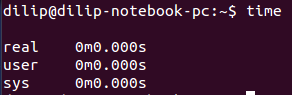
\includegraphics[scale=1]{3.png}
\caption{time: Get total program execution time in the shell}
\end{figure}
\section*{Lab Problems}
\begin{enumerate}
\item Familiarize yourself with the Linux commands and POSIX thread code given in this handout.
\item Solutions for Problems 1-2 on peak performance.
\item Using the basic Linux commands find the cache size, bandwidth number of processors on your system.
\item Write a C-code using POSIX threads to create an unbalanced load using sleep command and hello.c. The sample sleep times are given below:
\begin{enumerate}
\item thread-1: 1000 sec, thread-2: 5000 sec, thread-3: 20 sec, thread-4: 1200 sec.
\item Measure the total time taken for the complete execution of code with and without the additional sleep command.\\
Hint: You will require to include unistd.h for successful compilation.
\begin{figure}[!htp]
\centering
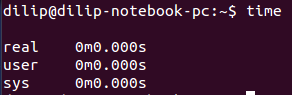
\includegraphics[scale=1]{3.png}
\caption{time: Get total program execution time in the shell}
\end{figure}
\end{enumerate}
\item Write a C-code using POSIX threads about matrix multiplication.
\begin{enumerate}
\item Take overall execution time measurement using time command for different application size and thread count for the serial and parallel code.
\item Observe gnome-system-monitor output as your fire up different thread counts.
\item Use the overall execution time measurements to plot and comment upon the speed-up.
\end{enumerate}
\end{enumerate}
\end{document}